\documentclass{report}

\usepackage[latin1]{inputenc}
\usepackage[english]{babel}
\usepackage{lmodern} %font
%\usepackage{url} % for clickable links
\usepackage[hidelinks]{hyperref} % for links in tableofcontent
\usepackage[top=3cm, bottom=4cm, left=4cm, right=4cm]{geometry} % for margins.
\usepackage[pdftex]{graphicx} % for images includes
\usepackage{titlesec}	% Remove the label ``chapter #''
\titleformat{\chapter}% But still display it in the ToC
  {\Large\bfseries} % format
  {}                % label
  {0pt}             % sep
  {\huge}           % before-code

\begin{document}

% the fancy title
\begin{titlepage}
\newcommand{\HRule}{\rule{\linewidth}{0.5mm}} % new command for the horizontal lines, change thickness here

\center % Center everything on the page
\textsc{\LARGE Halmstad's university}\\[1.5cm] % Name of your university/college
\textsc{\Large Advanced Oriented Object Programming}\\[0.5cm] % Major heading such as course name
%\textsc{\large Minor Heading}\\[0.5cm] % Minor heading such as course title
% title
\HRule \\[0.4cm]
{ \huge \bfseries Sound editor framework}\\[0.4cm] % Title of your document
\HRule \\[1.5cm]

% Authors
\begin{minipage}{0.4\textwidth}
\begin{flushleft} \large
\emph{Authors:}\\
R�mi \textsc{Gourdon}\\
Hichame \textsc{Moriceau} % Your name
\end{flushleft}
\end{minipage}
~
\begin{minipage}{0.4\textwidth}
\begin{flushright} \large
\emph{Supervisor:} \\
Dr. Veronica \textsc{Gaspes} % Supervisor's Name
\end{flushright}
\end{minipage}\\[4cm]
{\large \today}\\[3cm] % Date
\vfill % fill the rest of the page with whitespace
\end{titlepage}
% end of : fancy title


\tableofcontents % add summary


\chapter{Introduction}

Our framework offers to: synthesise, visualize and tweak sounds through different modifiers.
It comes with built-in generators, views, filters and effects, but, according to the project specifications, we did out best to make room for extensions.
Two implementations are provided, to demonstrate various ways of using it, and different manners of assembling its components.

The question of modularity was for us a top priority from day one. Indeed, audio creation is typically a domain where the possibilities are endless.
The sound generators can range from basic signal generators to complex synthesizer, either mimicking real instruments or creating completely new sounds.
The same goes for filters and effects, which can be as simple as low-pass and high-pass, delays, but also flangers, reverbs, etc.
For these modules, that we called modifiers, we also quickly realized that the possibility of adding several of them to the same sound would really expand the possibilities.

\chapter{Design}

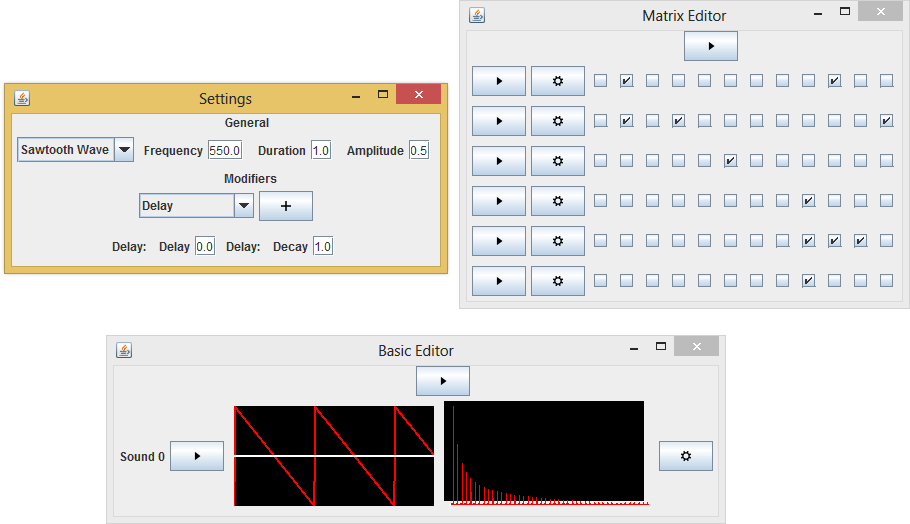
\includegraphics[scale=0.4]{global_view.png}

\section{Framework}

\subsection{Modularity}
The core of the framework is the class Sound. Everything depends on it, but we tried to limit the connections between the different parts of the framework, because we think it is generally a good practice. The model then is constructed in modules, that anyone can easily extends to its own needs.

Considering that we had to give the possiblity to derive both simple and more complex implementations from this framework, it was essential to keep the modules well separated.
As a result, we came up with a design where the only mandatory components to get a working application are a Sound object, a Generator and a Player.
It means that our framework could also be used as an external library, dedicated to the generation and playing of sounds.
Indeed, the data model relies on a simple array of samples, which could very well be integrated in any application requiring sound synthetis.
The generators and views by themselves could also be used as a third party library and integrated in other sound models.

\subsection{Extensibility}
When we started to think about the implementation, we wanted to give the user the ability to easily append new classes to any part of the framework.
The modularity is a first step toward this goal, the genericity of the superclasses and interfaces is the next one.
We tried not to put boundaries around the possible use cases.

\subsection{Flexibility}
An objective was to come up with a structure allowing the user to build upon it both command line utilities or graphical interfaces.
As the requirements were to provide a graphical user interface, we decided to design a flexible one.
It means that a client application could very well be working fully from the command line, though we didn't provide any example of this kind, because it wasn't our goal.
It could also be an hybrid, like the basic editor, which is taking its initial input from the console and then provides a graphical interface for further tweaking, playing and visualization of the signals.
Finally it can be fully graphical, as you can see in the matrix editor implementation, which provides a prebuild set of sounds, and the panels to adjusts their parameters further on.

\subsection{Reliability}
The Strategy pattern is used several times, for the choice of the signal, of the filter and the effect.
On this road, the necessity of using good design practices, and patterns, appeared rapidly.
We can see that we used the model/view/controller architecture, which is represented here with the Sound as the model, the View is obviously a view.

\section{Basic Editor}

\section{Matrix Editor}

The inspiration for the non-trivial application came from an embedded ActionScript application\footnote{http://www.hisschemoller.com/2009/step-sequencer-drum-machine/} allowing an easy creation of sound patterns.



\chapter{Testing}

\chapter{Some code we're proud of}

\chapter{Results}

\chapter{Sources}

\end{document}